% The pgf-soroban package
% Author: Alain Delmotte

\documentclass[]{article}
\usepackage{tikz}
\usepackage{pgf-soroban}
\usepackage{verbatim}

\begin{comment}
:Title: The pgf-soroban package
:Slug: pgf-soroban
:Tags: Graphs, Macro packages

The `pgf-soroban`_ package is a set of convenient macros for creating pictures
of a a soroban_. The soroban_ is a Japanese version of the abacus_. For details on
how to use the package, see the documentation_.

:Author: Alain Delmotte

.. _abacus: http://en.wikipedia.org/wiki/Abacus
.. _pgf-soroban: http://texcatalogue.sarovar.org/entries/pgf-soroban.html
.. _soroban: http://en.wikipedia.org/wiki/Soroban
.. _documentation: http://theory.uwinnipeg.ca/scripts/CTAN/graphics/pgf/contrib/pgf-soroban/pgf-soroban-doc.pdf

\end{comment}

\begin{document}

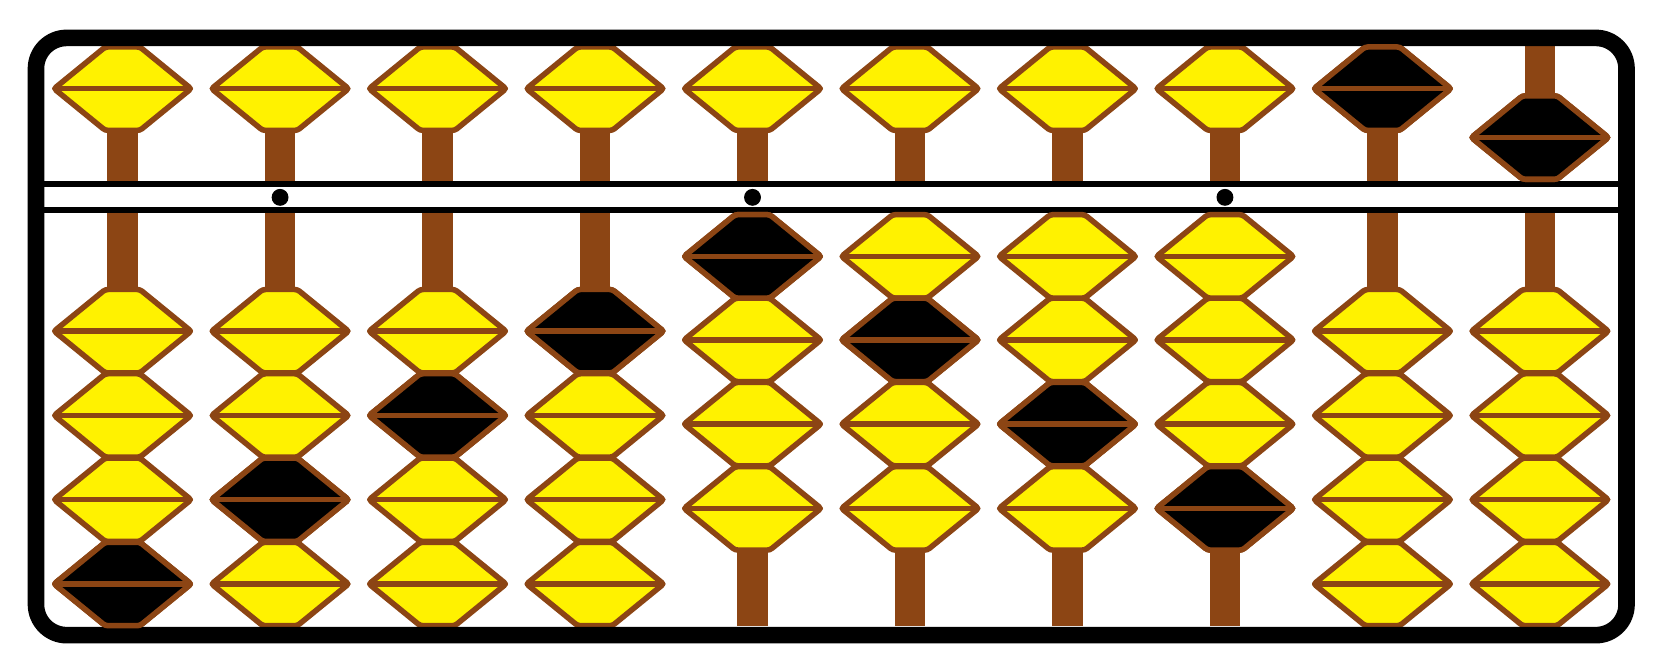
\begin{tikzpicture}
   \tige{1}{0}{0}
   \tige{2}{0}{1}       %<- here a dot: unit million
   \tige{3}{0}{0}       %<- here no dot: hundreds of thousands
   \tige{4}{0}{0}       %<- here no dot: tens of thousands
   \tige{5}{4}{1}       %<- here a dot: units thousands
   \tige{6}{4}{0}
   \tige{7}{4}{0}
   \tige{8}{4}{1}       %<- here a dot: units
   \tige{9}{0}{0}
   \tige{10}{5}{0}
   \cadre{10}
   \binoire{1}{1}{black}
   \binoire{2}{2}{black}
   \binoire{3}{3}{black}
   \binoire{4}{4}{black}
   \binoire{5}{5}{black}
   \binoire{6}{6}{black}
   \binoire{7}{7}{black}
   \binoire{8}{8}{black}
   \binoire{9}{9}{black}
   \binoire{10}{10}{black}
\end{tikzpicture}

\end{document}
